\section{\label{sec:interfaces} Crowdsourcing data collection}

In this section, we provide details regarding our the design of our annotation interfaces and the quality control measures we took.

\subsection{Language quality evaluation.}
Each human annotator was shown a short summary that was generated by a system from an article in the CNN/Daily Mail dataset or provided as a reference for that article.
The annotators were then asked to (a) provide Likert scale ratings of the summary on multiple facets (fluency, redundancy and overall quality) and (b) perform post-edits to correct any errors (\reffig{lqual-interface}).

\paragraph{Interface design choices.}
We found that using a five-level Likert scale increased annotator variance as annotators relative to a three-level Likert scale.
Annotators were provided specific cues to calibrate their Likert ratings through a tutorial and were reminded of these cues through tooltips on the rating buttons (see \reffig{lqual-tutorial} for an example).
If the annotators rated a summary as lacking along any facet, they were then forced to perform post-edits to ``improve [its] quality as much as possible''.
We found that forcing annotators to provide post-edits on examples significantly decreased the annotator variance even on the Likert ratings.

\begin{figure*}
  \begin{subfigure}{\textwidth}
    \centering
    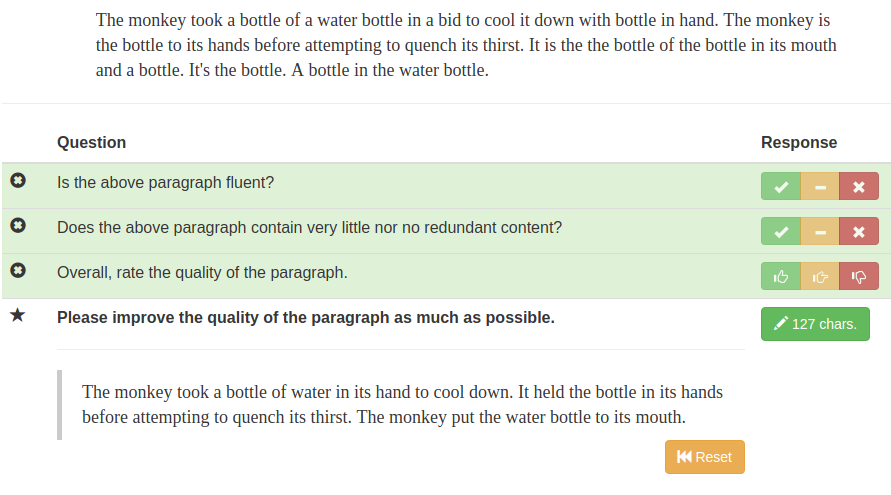
\includegraphics[width=0.8\textwidth]{figures/edit}
    \caption{\label{fig:lqual-interface}}
  \end{subfigure}
  \begin{subfigure}{\textwidth}
    \centering
    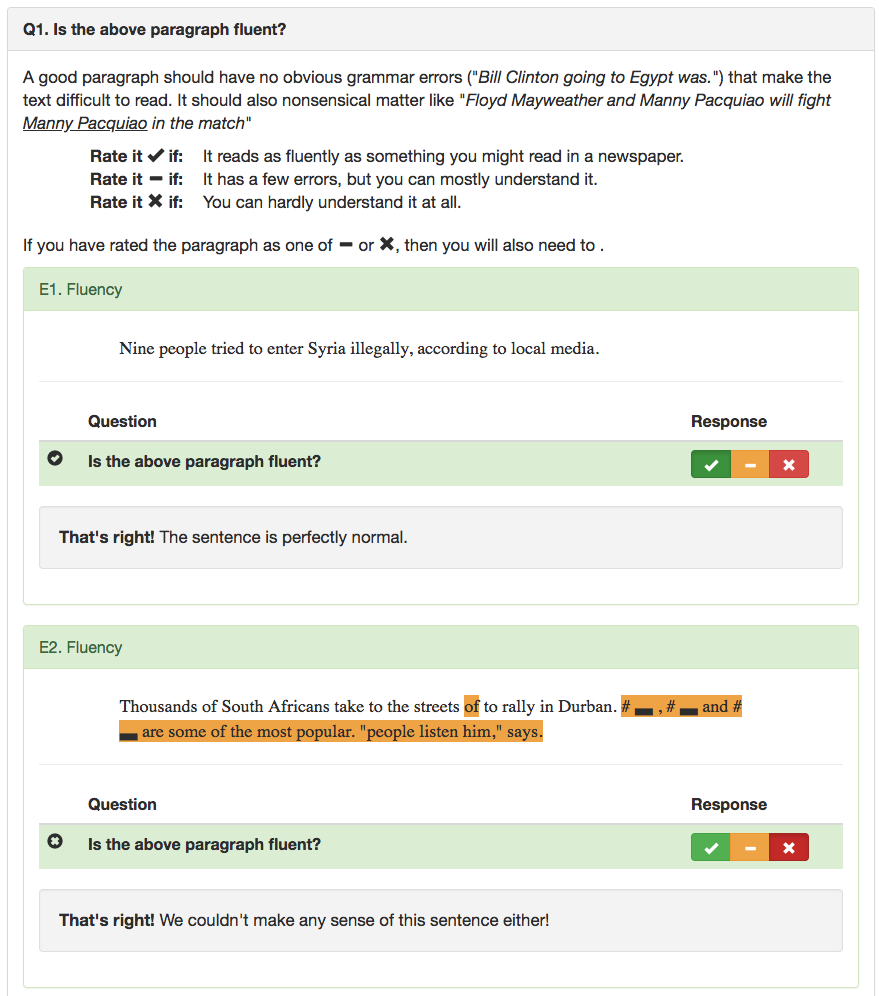
\includegraphics[width=0.8\textwidth]{figures/lqual_tutorial}
    \caption{\label{fig:lqual-tutorial}}
  \end{subfigure}
  \caption{Screenshot of the (a) interface and (b) instructions used by crowdworkers for the language quality evaluation task on the CNN/Daily Mail dataset.}
\end{figure*}

\begin{figure*}
  \begin{subfigure}{\textwidth}
    \centering
    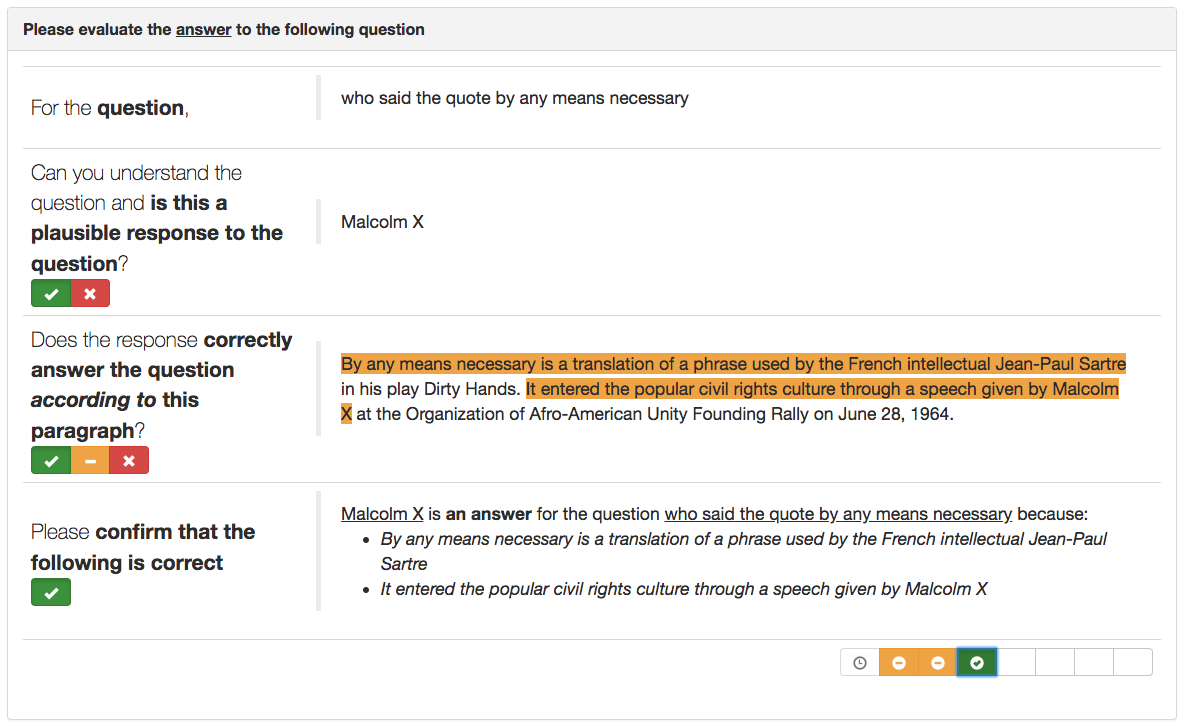
\includegraphics[width=0.8\textwidth]{figures/msmarco_interface}
    \caption{\label{fig:msmarco-interface}}
  \end{subfigure}
  \begin{subfigure}{\textwidth}
    \centering
    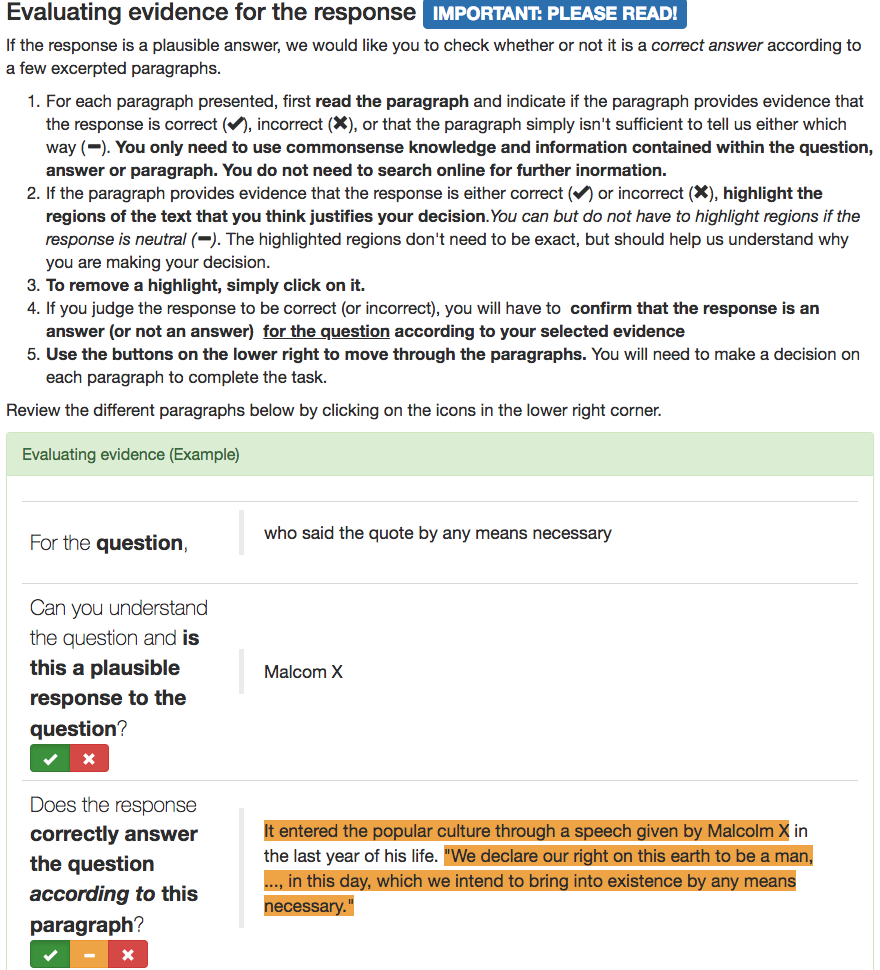
\includegraphics[width=0.8\textwidth]{figures/msmarco_tutorial}
    \caption{\label{fig:msmarco-tutorial}}
  \end{subfigure}
  \caption{Screenshot of the (a) interface and (b) instructions used by crowdworkers for the answer correctness evaluation task on the MS MARCO dataset.}
\end{figure*}

Following the recommendations of \citet{liu2016effective}, we forced annotators to complete an interactive tutorial containing 10 questions each before beginning the task (\reffig{lqual-tutorial}).
The tutorial provided guidelines and examples on how to rate each facet (fluency, redundancy and overall quality) and tested whether they were able to identify and correct language errors using the post-editing interface.
The tutorial took about 5--6 minutes to complete and annotators were paid a one-time bonus of \$0.75 on completion.

We initially included additional questions to assess focus, coherency and referential clarity adapted from the DUC evaluation guidelines~\citep{dang2006overview}, but found that annotators were unable to reliably identify these errors in the short summaries.
We also experimented with asking annotators to highlight language errors in the text to justify their ratings, but again found that annotators were unable to localize these errors reliably.

\paragraph{Quality control measures.}

We initially attempted to use attention-check examples for the Likert rating questions, but found that the ratings on these examples were themselves quite subjective and hence were not a reliable signal to reject work.
Instead, we found that requiring post-edits to summaries significantly reduced spam.
Additionally, we rejected annotators who took too little time to complete the task, had very low agreement rates on the Likert questions or had edits that were consistently shorter than 5 characters to prevent spam.

\subsection{Answer correctness evaluation.}
Each annotator was shown a question from the MS MARCO dataset and an answer that was generated by a system or provided as a reference answer from the dataset.
The annotators were then asked to (a) rate if the question made sense and the answer was plausibly correct and (b) asked to identify which paragraphs provided in the dataset justified the answer (\reffig{msmarco-interface}).

\paragraph{Interface design choices.}
We found that some of the questions in the MS MARCO dataset were extremely ambiguous (e.g.\ ``metatarsal what causes'') and some system responses were implausible (e.g\ ``monogenic bone diseases'', for the question ``what genes cause osteoporosis'').
In these cases, annotators expressed confusion if they were forced to judge if the response was correct or incorrect.
We resolved this confusion by first asking annotators if the question made sense and if system response was even plausible.

In early pilots, we found that annotators often rated a paragraph that correctly answered the question but was unrelated to the system response to be ``correct''.
We were able to resolve this problem by asking annotators to double-check their work (see the last question in \reffig{msmarco-interface} for an example).

Once again, we forced annotators to complete an interactive tutorial containing eight questions each before beginning the task (\reffig{msmarco-tutorial}).
The tutorial also took about 5--6 minutes to complete and annotators were paid a one-time bonus of \$0.75 on completion.

\paragraph{Quality control measures.}
We found that requiring annotators to provide justification spans significantly spam.
Additionally, we rejected annotators who took too little time to complete the task or had very low agreement rates on the answer correctness.

%\subsection{Round-trip machine translation quality}
%For an independent source of language quality evaluations, we used the annotations collected by \citet{lau2017grammaticality} to evaluate the level of ``acceptability'' of a sentence.
%This dataset contains of 2,500 sentences derived from the BNC Consortium (2007) and 2,500 sentences from Wikipedia.
%Each sentence was then translated into one of four languages (Spanish, Norwegian, Chinese and Japanese) using Google Translate and then translated back into English to be evaluated by many different human annotators.
%It is observed that performing round-trip machine translation through different languages degrades the quality of of the resulting sentence to different degrees.
%For purposes of this benchmark, we consider each language as a separate system for evaluation.
%
